\documentclass{article}
\usepackage{enumerate}
\usepackage{algorithm}
\usepackage{algorithmic} % pesudo code

\usepackage{hyperref}

\usepackage{tikz}
\usetikzlibrary{positioning,shapes,arrows}
\tikzset{
    %Define standard arrow tip
    >=stealth',
    %Define style for boxes
    punkt/.style={
           rectangle,
           rounded corners,
           draw=black, very thick,
           text width=6.5em,
           minimum height=2em,
           text centered},
    % Define arrow style
    pil/.style={
           ->,
           thick,
           shorten <=2pt,
           shorten >=2pt,}
}

\usepackage{amsmath,amsfonts,amsthm} % Math packages
\usepackage{graphicx}
\usepackage{caption}
\usepackage{subcaption}

\newcommand{\norm}[1]{\left\lVert #1 \right\rVert}
\newtheoremstyle{quest}{\topsep}{\topsep}{}{}{\bfseries}{}{ }{\thmname{#1}\thmnote{ #3}.}
\theoremstyle{quest}
\newtheorem*{question}{Question}
\begin{document}
\begin{question}[1]
\end{question}
\begin{enumerate}[a.]
\item
~\\
\begin{tabular}{ll}
states & A class-to-room assignment.\\
operators & Move one class to a different room. (swap classes, if time conflict occurs)\\
start state & current class-to-room assignment (given by register office)\\ 
goal test & A valid class-to-room assignment \\
& (each class is assigned to an acceptable classroom without conflict.)
\end{tabular}
\item
Yes. Because the problem requires using the smallest number of changes, which can be obtained by minimize the search depth.
\item
$b = |R|^{|C|}$, where $|R|$ is the number of rooms, $|C|$ is the number of classes. 
\item
$O(b^d)$, where $b$ is the branching factor, $d$ is the search depth. 
\item
Yes. Suppose D, E, F are 3 classes in C with size 30, 40, 100 respectively, and $R_1$, $R_2$, $R_3$ are 3 rooms in R with size 40, 20, 100. Class D conflicts with both E and F, while E and F are compatible . The start state is as the following figure shows: \\
~\\
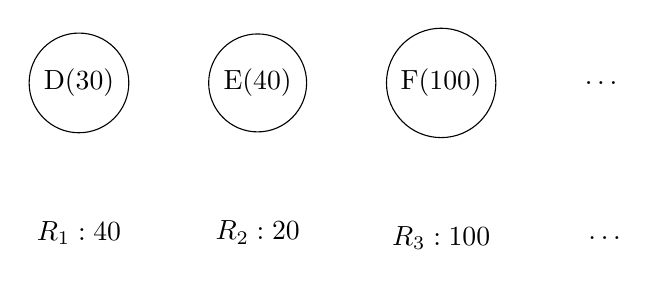
\begin{tikzpicture}
\node [circle,draw] (a) {D(30)};
\node [circle,draw,right=of a] (b) {E(40)};
\node [circle,draw,right=of b] (c) {F(100)};
\node [right=of c] (d) {$\ldots$};
\node [below=of a] (e) {$R_1: 40$};
\node [below=of b] (f) {$R_2: 20$};
\node [below=of c] (g) {$R_3: 100$};
\node [right=of g] (h) {$\ldots$};
%\path (a)
%edge[pil, <->, bend left=45] node[auto] {cycle} (b);
\end{tikzpicture}

There are multiple ways to make a valid assignment use $R_1$, $R_2$, $R_3$ for D, E, and F. You can just move E to $R_3$, that makes a valid assignment. You can also swap D and E (due to time conflict), but D still not satisfied, $D.size >R_2.size$. Then you can swap D and F, that will make F(at $R_2$) invalid. We can move F to $R_1$, then swap D and F with E, that makes the same valid assignment.  Such multiple solutions to part of the search causes duplicate states in different branches.
\item
\begin{align}
h(n) &= \sum\limits_{i=1}^{N} f(i) \\
f(i) &=
\begin{cases}
C(i).size - R(C(i)).size. &  \text{if } C(i).size > R(C(i)).size\\
 0   & \text{otherwise}
\end{cases}
\end{align}
where $N$ is the number of classes, $C(i)$ denotes class $i$ and $R(C(i))$ denotes its current assigned room.

If the problem is relaxed by ignoring time interval, then h(n) gives the shortest solution. So h(n) is an admissible heuristic.
\end{enumerate}
\begin{question}[2]
\end{question}
\begin{enumerate}[a.]
\item
~\\
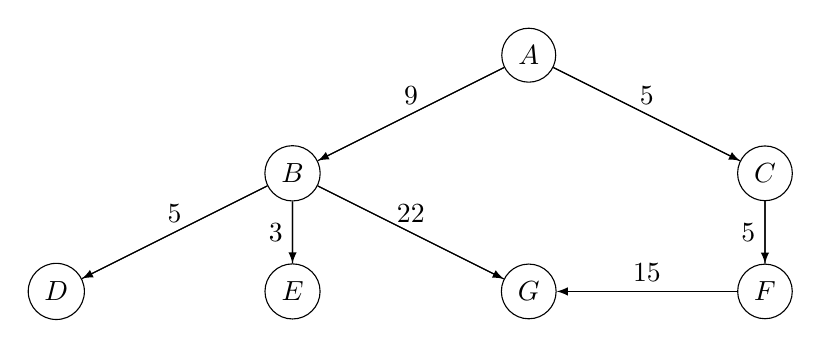
\begin{tikzpicture}[level/.style={sibling distance=60mm/#1}]
\node [circle,draw] (a) {$A$}
	child {node [circle,draw] (b) {$B$}
		child {node [circle,draw] (d) {$D$}}
		child {node [circle,draw] (e) {$E$}}
		child {node [circle,draw] (g) {$G$}}	
	}
	child {node [circle,draw] (c) {$C$}
		child {node [circle,draw] (f) {$F$}}
		};
\path (a) edge[-latex] node [midway, above] {9} (b)
(a) edge[-latex] node [midway, above] {5} (c)
(b) edge[-latex] node [midway, above] {5} (d)
(b) edge[-latex] node [midway, left] {3} (e)
(b) edge[-latex] node [midway, above] {22} (g)
(c) edge[-latex] node [midway, left] {5} (f)
(f) edge[-latex] node [midway, above] {15} (g);
\end{tikzpicture}
\item
$A\rightarrow B \rightarrow D \rightarrow E \rightarrow G \rightarrow C \rightarrow F \rightarrow G$
\item
$A \rightarrow B \rightarrow C \rightarrow D \rightarrow E \rightarrow G \rightarrow F \rightarrow G$
\item
$A \rightarrow A \rightarrow B \rightarrow C \rightarrow A\rightarrow B \rightarrow D \rightarrow E \rightarrow G \rightarrow C \rightarrow F \rightarrow A\rightarrow B \rightarrow D \rightarrow E \rightarrow G \rightarrow C \rightarrow F \rightarrow G$
\item
$A\rightarrow C \rightarrow F \rightarrow B \rightarrow G$
\item
$A\rightarrow C \rightarrow F \rightarrow G$
\end{enumerate}

\begin{question}[3]
\end{question}
\begin{enumerate}[viii.]
\item
Detect whether there's a cat in a given photo?

Yes. 

Object Classificaion/Detection make huge progress in recent years, thanks to novel discriminative features \href{ourses.northwestern.edu/webapps/portal/frameset.jsp}{BoW} and \href{http://lear.inrialpes.fr/people/triggs/pubs/Dalal-cvpr05.pdf}{HOG}(Visual Bag of Words, Histogram of Oriented Gradient), invariant detector model \href{http://www.cs.berkeley.edu/~rbg/latent/}{DPM} (Deformable Part-based Model), and massive avaliable data from web. Since cat's body is deformable (walking, lying, Jumping etc.), and it has discriminative feature in different body part, we can fulfill this task very well by using feature mentioned above with DPM.

\begin{figure}[htb!]
\centering
\includegraphics[width=1.1\textwidth]{cat.jpg}
\caption{Some result of cat detection by DPM. Red bouding box denotes a cat detection, blue bounding boxes denotes a cat part detection. (Image cliped from lecture note of MIT CSAIL 6.869: Advances in Computer Vision)}
\end{figure}

In VOC (Visual Object Classes) 2012 challenge the best algorithm for detecting cat in images achieved 89.3\% average precision (that's the average precision of the ROC curve). 

Here is the link, the first half of the page is a leaderboard of different submitted algorithm, the second half contians brief descriptions of these algorithms and link to published paper.

\url{http://host.robots.ox.ac.uk:8080/leaderboard/displaylb_dt.php?cls=cat&challengeid=11&compid=1}



\end{enumerate}
\begin{question}[4]
\end{question}
Extra Credit.

All my code is in ./qualification, with each problem a subfolder named by the problem's name.

I answered all the 4 problems and passed all the test except got a time expired for problem C's large input (that's as expected). I used DFS for problem C, maybe it lacks some termination condition, but I think score 66/90 is enough, and hope to see other's solutions after this round.
\end{document}
